\section{Evaluation}\label{sec:eval}

We ran four open-weight models on two GPU generations with request traces from a public chat service~\cite{haddadin2025traces}.
For every request we also measured the same prompt alone on an idle device, which serves as the reference.
Earlier studies measured the energy of training~\cite{strubell2019energy,patterson2021carbon,luccioni2023bloom} and of inference as a whole~\cite{samsi2023words}, and serving systems share memory between requests~\cite{kwon2023paged}.

\begin{table}[t]
  \caption{Attributed energy per request against isolated reference runs.}
  \label{tab:results}
  \begin{tabular}{lrrr}
    \toprule
    Model & Parameters & Median error & Coverage \\
    \midrule
    Model A & 8B  & 4.8\,\% & 95.1\,\% \\
    Model B & 13B & 5.9\,\% & 94.6\,\% \\
    Model C & 34B & 6.4\,\% & 93.8\,\% \\
    Model D & 70B & 7.2\,\% & 93.0\,\% \\
    \bottomrule
  \end{tabular}
\end{table}

Table~\ref{tab:results} shows the median error per request.
Coverage is the share of the measured energy that \sysname{} attributes to a request.
The rest is idle power and the work of the serving framework itself.

\begin{figure}[t]
  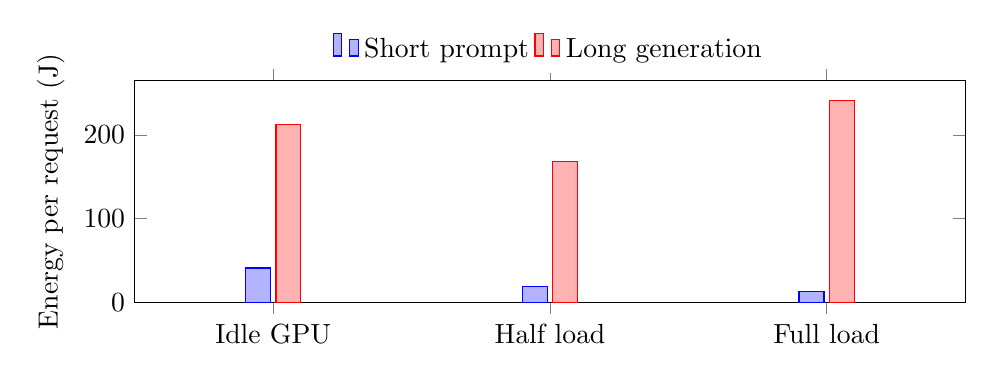
\begin{tikzpicture}
    \begin{axis}[
        ybar, width=\columnwidth, height=4.4cm, ymin=0, bar width=9pt,
        ylabel={Energy per request (J)},
        symbolic x coords={Idle GPU, Half load, Full load}, xtick=data,
        enlarge x limits=0.25,
        legend style={at={(0.5,1.03)}, anchor=south, legend columns=2, draw=none},
      ]
      \addplot coordinates {(Idle GPU, 41) (Half load, 19) (Full load, 13)};
      \addplot coordinates {(Idle GPU, 212) (Half load, 168) (Full load, 241)};
      \legend{Short prompt, Long generation}
    \end{axis}
  \end{tikzpicture}
  \caption{The same two requests under three load levels.}
  \label{fig:load}
\end{figure}

Figure~\ref{fig:load} shows why a per-request figure needs the load around it.
A short prompt gets cheaper as the batch fills, because the fixed cost of each decoding step is shared.
A long generation gets more expensive at full load, because it keeps the batch open while new requests queue behind it.
